	\paragraph{QuizziPedia::Front-End::ModelViews::FillingQuestionnaireModelView}
	
	\label{QuizziPedia::Front-End::ModelViews::FillingQuestionnaireModelView}
	
	\begin{figure}[ht]
		\centering
		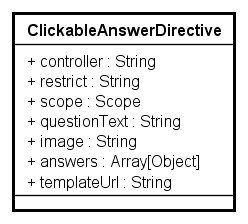
\includegraphics[scale=0.5,keepaspectratio]{UML/Classi/Front-End/QuizziPedia_Front-end_Templates_ClickableAnswerTemplate.png}
		\caption{QuizziPedia::Front-End::ModelViews::FillingQuestionnaireModelView}
	\end{figure} \FloatBarrier
	
	\begin{itemize}
		\item \textbf{Descrizione}: classe di tipo modelview la cui istanziazione è contenuta all'interno della variabile di ambiente \$scope di \textit{Angular.js\ped{G}}. All'interno di essa sono presenti le variabili e i metodi necessari per il \textit{Two-Way Data-Binding\ped{G}} tra la view \texttt{FillingQuestionnaireView} e il controller \texttt{FillingQuestionnaireController};
		\item \textbf{Utilizzo}: viene utilizzata per effettuare il \textit{Two-Way Data-Binding\ped{G}} tra la view \texttt{FillingQuestionnaireView} e il controller \texttt{FillingQuestionnaireController} rendendo disponibili variabili e metodi;
		\item \textbf{Relazioni con altre classi}: 
		\begin{itemize}
			\item \textit{OUT} \texttt{FillingQuestionnaireView}: view principale per la compilazione del questionario. Conterrà i vari templates di ogni domanda appartenente al questionario; 
			\item \textit{OUT} \texttt{FillingQuestionnaireController}: questa classe permette di gestire la compilazione del questionario;
		\end{itemize}
		\item \textbf{Attributi}: 
		\begin{itemize}
			\item \texttt{+ quiz: Object} \\ Oggetto contenente al suo interno i seguenti campi:
			\begin{itemize}
				\item \texttt{+ title: String} \\ Attributo che rappresenta il titolo del questionario;
				\item \texttt{+ argument: String} \\ Attributo che rappresenta l'argomento del questionario;
				\item \texttt{+ keywords: Array[String]} \\ \texttt{array} di stringhe che contiene le parole chiave del questionario;
				\item \texttt{+ questionNumber: String} \\ Attributo che rappresenta il numero progressivo della domanda attuale;
				\item \texttt{+ numberOfQuestions: String} \\ Attributo che rappresenta il numero di domande.
			\end{itemize}	
		\end{itemize}
		\item \textbf{Metodi}: 
		\begin{itemize}
			\item \texttt{+} \texttt{loadNextQuestion(question: QuestionItemModel): void}: \\ Metodo che invoca l'evento per visualizzare la domanda successiva del quiz tramite QuestionController; \\
			\textbf{Parametri}:
			\begin{itemize}
				\item \texttt{question: QuestionItemModel} \\
				Parametro contenente un riferimento all'oggetto di tipo \texttt{QuestionItemModel}.
			\end{itemize}
			\item \texttt{+} \texttt{loadPreviousQuestion(question: QuestionItemModel): void}: \\ Metodo che invoca l'evento per visualizzare la domanda precedente del quiz tramite QuestionController; \\
			\textbf{Parametri}:
			\begin{itemize}
				\item \texttt{question: QuestionItemModel} \\
				Parametro contenente un riferimento all'oggetto di tipo \texttt{QuestionItemModel}.
			\end{itemize}
		\end{itemize}
	\end{itemize}
	
	